\Aufgabe[e]{Volumen und Masse}{
Gegeben sei der Körper
$$
\mathbf{K} = \left\{ \vec x = \begin{pmatrix} x\\y\\z \end{pmatrix} \in \mathbb{R}^3 :
z \leq \sqrt{x^2 +y^2}, \, 0 \leq z \leq 2\right\}.
$$
\begin{abc}
\item Skizzieren Sie den dreidimensionalen Körper $\mathbf{K}$.
\item Bestimmen Sie das Volumen des Körpers durch Integration in Zylinderkoordinaten.
\item Gegeben sei die Dichtefunktion
$$
\rho(x,y,z) =  x + 2y +z^2.
$$
      Bestimmen Sie die Masse des Körpers, die durch
      
$$
M = \int_{K} \rho(\vec x) \mathrm{d} \vec x
$$
gegeben ist.      
\end{abc}
}

\Loesung{
\begin{abc}
\item 
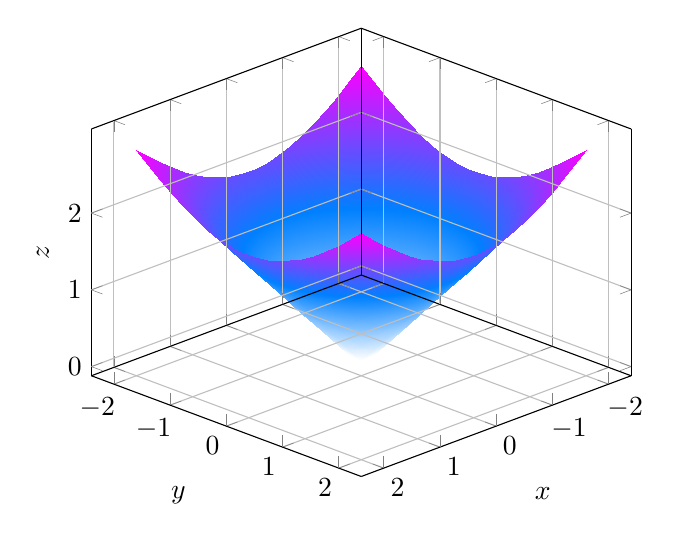
\begin{tikzpicture}
  \begin{axis}[
    view={135}{30},
    xlabel={$x$}, ylabel={$y$}, zlabel={$z$},
    domain=-2:2,
    y domain=-2:2,
    samples=20,
    samples y=20,
    axis on top,
    z buffer=sort,
    colormap/cool,
    enlargelimits=true,
    grid=major,
    xtick={-2,-1,0,1,2},
    ytick={-2,-1,0,1,2},
    ztick={0,1,2},
  ]
    \addplot3[
      surf,
      shader=interp,
      opacity=1,
    ]
    {sqrt(x^2 + y^2)};
  \end{axis}
\end{tikzpicture}
%
\item
Wir transformieren von kartesischen Koordinaten in Zylinderkoordinaten.
$$
x = r \cos(\varphi), \quad
y = r \sin(\varphi), \quad
z = z
$$
Die Integrationsgrenzen sind dann gegeben durch
$$ 
0 \leq r \leq 2 , \quad r \leq z \leq 2, \quad 0 \leq \varphi \leq 2\pi 
$$
Die Jacobi-Determinate ist $r$.

Damit erhalten wir das Integral.
\begin{align*}
V &= \int_0^2 \int_r^2 \int_0^{2\pi} r \mathrm{d} \varphi  \mathrm{d} z  \mathrm{d} r \\
&= 2\pi \int_0^2 \int_r^2 r  \mathrm{d} z  \mathrm{d} r \\
&= 2\pi \int_0^2 rz\Big|_r^2  \mathrm{d} r\\
&= \int_0^2 (2-r)r \d r\\
&= 2\pi\left( \frac{2r^2}{2}\Big|_0^2 - \frac{r^3}{3}\Big|_0^2 \right)\\
&= 2\pi (4-\frac{8}{3})\\
&= \frac{8}{3} \pi
\end{align*}
Damit ist das Volumen des gegebenen Kegels $\frac{8}{3}\pi$.

\item
\begin{align*}
M &= \int_K x + 2y +z^2 \mathrm{d} V  \\
&= \int_0^2 \int_r^2 \int_0^{2\pi} (r\cos(\varphi) +2r\sin(\varphi) +z^2)r  \mathrm{d} \varphi  \mathrm{d} z \mathrm{d} r\\
&= \int_0^2 \int_r^2 \left(r\sin(\varphi)\Big|_0^{2\pi}- 2r\cos(\varphi)\Big|_0^{2\pi}+ z^2\varphi\Big|_0^{2\pi}\right)r \mathrm{d} z  \mathrm{d} r\\
& = \int_0^2 \int_r^2 2\pi z^2r  \mathrm{d}z  \mathrm{d}r\\
& = \int_0^2 2\pi r\frac{z^3}{3}\Big|_r^2  \mathrm{d} r\\
& = \int_0^2 \frac{16\pi r}{3} - \frac{2\pi r^4}{3}  \mathrm{d} r\\
& = \frac{8 \pi r^2}{3}\Big|_0^2 -\frac{2\pi r^5}{3} \Big|_0^2 \\
& = \frac{32 \pi}{5}
\end{align*}
\end{abc}
}

\ErgebnisC{analysIntgKegel001}{
\begin{abc}
\item $V = \frac{8}{3} \pi$
\item $M = \frac{32 \pi}{5}$
\end{abc}
}
